\documentclass{proposal}
\usepackage{graphicx}
\usepackage[square,numbers]{natbib}
\usepackage{listing}
\usepackage[labelfont=bf, font=small]{caption}
\usepackage{minted}
\usepackage{chngcntr}
\usepackage[hyphens]{url}
\usepackage{tikz}
\usepackage{pgfgantt}
\usepackage{rotating}
\usepackage{hyperref}

\setminted{frame=lines, linenos, autogobble, breaklines}

\begin{document}

    \counterwithin{listing}{section}
    \counterwithin{figure}{section}


%%%%%%%%%%%%%%%%%%%%%%%%%%%%%%%%%%%%%%%%%%%%%%%%%%%%%%%%%%%%%%%%%%%%%%%%%%%%%%%%%%%%%%%%%%%%%%%%%%%%%%%%%%%%%%%%%%%%%%%%


    \title{ptr-tidy: Automatic refactoring of raw pointers in C++}
    \author{Artem Usov\\ 2296905U}
    \date{18 December 2020}
    \maketitle
    \tableofcontents
    \newpage


%%%%%%%%%%%%%%%%%%%%%%%%%%%%%%%%%%%%%%%%%%%%%%%%%%%%%%%%%%%%%%%%%%%%%%%%%%%%%%%%%%%%%%%%%%%%%%%%%%%%%%%%%%%%%%%%%%%%%%%%


    \section{Introduction}\label{sec:intro}

    \subsection{Difficulties with Memory Management}\label{subsec:difficulties-with-memory-management}

    Systems programming often involves memory management, that is requesting memory from operating system to be used and managed by the program.
    This is done when the amount of memory that we need cannot be known at the time of compilation of the program.
    However doing so creates the opportunity for memory safety errors~\cite{Dhurjati2003} which are notoriously challenging to avoid.

    \emph{How challenging one might ask?}

    In a presentation by Matt Miller, a security engineer at Microsoft, it is shown that around 70\% of their vulnerabilities that are addressed through a security updates are due to memory safety issues~\cite{Miller2019}.
    In another presentation at the Linux Security Summit it is shown that in several other top projects such as Firefox, macOS, Ubuntu and Android all had over half of their CVEs~\footnote{\url{https://cve.mitre.org/}} attributed to issues with memory safety~\cite{Gaynor2020}.
    This is at industry-leading companies who are renowned for hiring top talent.
    Such memory safety vulnerabilities can be exploited, and due to new regulations such as the GDPR, these issues are more commonly exposed to the general public and punished by regulators.
    An example is a fine of £20m for a British Airways data breach by the British Information Commissioner's Office~\cite{ICO2020}.

    \subsection{Possible Solutions to Memory Management}\label{subsec:possible-solutions-to-memory-management}

    Memory safety errors occur in languages that place the task of memory management with the programmer, such as C and C++.
    However simply not using these languages is not an option since their unmanaged nature makes them highly performant, and therefore the best option for systems such as a web browser.

    \emph{What can be done then to address this issue?}

    Engineers at both Microsoft~\cite{Thomas2019} and Mozilla~\cite{Hostfelt2019} converge on Rust~\cite{Balasubramanian2017} as a possible solution.
    Rust is a systems language that offers similar performance as C and C++~\cite{Lin2016}, however its linear type system and memory ownership model also guarantee memory safety.
    The rewriting of a program in a new language, namely from C++ to Rust, is a colossal undertaking, especially given that Rust has a reputation for being difficult to learn.
    We therefore propose an alternative partial solution to this problem.


%%%%%%%%%%%%%%%%%%%%%%%%%%%%%%%%%%%%%%%%%%%%%%%%%%%%%%%%%%%%%%%%%%%%%%%%%%%%%%%%%%%%%%%%%%%%%%%%%%%%%%%%%%%%%%%%%%%%%%%%


    \section{Statement of Problem}\label{sec:statement-of-problem}

    \subsection{Using Smart Pointers for Memory Management}\label{subsec:using-smart-pointers-for-memory-management}

    Generally pointers are used to give the program access to a resource that cannot be directly included in the program itself, such as allocated memory or a file.
    However Stroustrup claims that pointers to objects allocated on the free store are dangerous and a \emph{plain old pointer}, or raw pointer as we will refer to them, should not be used to represent ownership~\cite{Stroustrup2018}.

    \begin{listing}
        \inputminted{c++}{code/manual-leak.cpp}
        \caption{Example of memory leaks using manual management. Lines 4 and 5 show how the memory allocated on line 2 will never be freed since the control flow of the function is interrupted before we reach line 7 and free the memory}
        \label{lst:manual-leak}
    \end{listing}

    % TODO insert some information about heap vs stack

    In \autoref{lst:manual-leak} we can see that when using a raw pointer, there are two cases in which the programmer will never free the allocated memory.
    Instead we can use \emph{smart pointers}~\cite{Dimov2003} and the concept of \emph{RAII (Resource Acquisition Is Initialisation)}~\cite{Stroustrup2000} to create resource handles which automatically eliminate resource leaks with no, or very little added overhead.
    The first type of smart pointer are \emph{unique pointers} which have only a single unique owner at any time.
    We can therefore fix the previous example in which we leak memory by using a unique pointer, as can be seen in \autoref{lst:first-example-unique}.
    In the comments of \autoref{lst:first-example-unique}, we can see all the locations where the control flow exits the scope where \emph{p} is defined and where the compiler will automatically insert delete statements, now ensuring that the resource will never get leaked.
    The ownership of a unique pointer can be transferred between variables using \mintinline{c++}{std::move} which moves the ownership from one variable to another, making the original reference invalid.

    \begin{listing}
        \inputminted{c++}{code/first-example-unique.cpp}
        \caption{Example of using a unique pointer to manage memory. Note how the programmer no longer has to specify to manually delete the pointer as in \autoref{lst:manual-leak}, and how the compiler can detect that on lines 4, 5 and 7 the variable $p$ leaves the scope and therefore needs to be freed. The compiler will automatically insert these delete statements during compilation.}
        \label{lst:first-example-unique}
    \end{listing}

    The second type of smart pointer are \emph{shared pointers} which are used for resources which may not necessarily have a single unique owner and so several owners \emph{share} ownership to the resource.
    Reference counting~\cite{Collins1960} is used to ensure that after the last owner loses access to the resource, it will finally be freed.
    Shared pointers are suitable to be used in most situations and such reference counted pointers are used by default for all values in the Python and Swift languages.

    \subsection{Do Smart Pointer Solve Memory Management?}\label{subsec:do-smart-pointer-solve-memory-management?}

    It would appear then that smart pointers could solve most of our memory management issues, but they were only introduced in the C++11 standard.
    The C++ standards (\textit{versions}) before then did not have these language features, with older programs being written predominantly in the C++98 or C++03 standard.
    There remain many such called \emph{legacy} programs which have not upgraded to newer standards, and even then the programmer can choose not to utilise smart pointers in their code.

    \subsubsection{Research Aim}\label{subsubsec:reseach-aim}

    % TODO find reference of how much old code is in production

    We therefore propose to create an automatic refactoring tool \emph{(ptr-tidy)}, that performs static analysis on C++ code and aims to refactor usage of raw pointers into smart pointers.
    It will involve a conservative analysis that first and foremost tries to identify raw pointers that only have a single unique owner at any point in the program.
    These will be refactored into unique pointers.
    If this cannot be guaranteed, then a more conservative refactoring to a shared pointer will be applied.
    We aim to apply automatic refactoring without changing the runtime behaviour compared to the original programs, which we believe will be possible given that C++ language standards are backwards-compatible to a high degree~\cite{Winters2020}.

    We use the term refactoring as this is one most familiar to programmers to convey a change in code that does not change its behaviour, but improves its the quality or maintainability.
    However, our work aligns more closely with the term \emph{source code rejuvenation}, as defined by \citet{Pirkelbauer2010}.
    This is because we exactly aim to replace outdated coding patterns with newer, higher-level abstractions, as well as fitting the notion that this tool would be applied once to a codebase, rather than be a reoccurring task.
    The two terms can be used interchangeably in the context of this paper, however we will exclusively use the term refactoring for simplicity.

    \subsection{Research Questions}\label{subsec:research-questions}

    We outline below the research questions we would like to answer alongside developing the tool.
    Namely we would like to answer the question of whether such a tool can truly improve C++ code by seeing if the tool can be used outside small examples on larger existing programs, as well as if the refactored results produce code which can be compiled and can be judged to be better.
    Secondly, if the tool is able to do this, we want to evaluate how well the tool performs by analysing the effectiveness of the analysis algorithms.

    \emph{RQ1: Can the translation of raw pointers into smart pointers be used to make existing C++ code more modern, safe and extendable?}

    \emph{RQ2: Can the tool reliably identify situations in which unique pointers should be used?}


%%%%%%%%%%%%%%%%%%%%%%%%%%%%%%%%%%%%%%%%%%%%%%%%%%%%%%%%%%%%%%%%%%%%%%%%%%%%%%%%%%%%%%%%%%%%%%%%%%%%%%%%%%%%%%%%%%%%%%%%


    \section{Background Survey}\label{sec:background-survey}

    In this section we will look into frameworks, design patterns and algorithms that we will use to enable us to read and refactor C++ code and to identify the locations where we can apply our refactorings.
    We also look into existing memory safe languages, garbage collection as a solution for automated memory management as well as related existing research.

    \subsection{Clang and LLVM}\label{subsec:clang-and-llvm}

    C++ as a language is enormous, and the first capability our tool will need is to be able to parse (\textit{read}) C++ code.
    Doing this ourselves would be an undertaking that would surely span longer than the time span of the whole project, therefore it was decided early to use an existing parser.
    The most capable and mature C++ parsers will naturally be the parsers used by the most popular compilers.
    This leaves us therefore with a choice between GCC~\footnote{\url{https://gcc.gnu.org/}} and Clang~\footnote{\url{https://clang.llvm.org/}}.
    The literature~\cite{Duffy2014} is fairly clear on the fact that the design of GCC makes it unsuitable for integration with other projects.
    Clang on the other hand allows us access to the Clang abstract syntax tree (AST) and parser internals via a standard API such as consumers and visitors.

    Clang is a front-end to the LLVM framework~\cite{Lattner2004} and transforms C++ code into the LLVM intermediate representation (IR).
    The LLVM IR is a language-independent, static single assignment (SSA)~\cite{Rosen1988} representation of the program and will be the target on which we apply our analysis to identify refactoring opportunities.
    We believe this choice will lead to several benefits in terms of the analysis power and future usage of the project:
    \begin{itemize}
        \item First, the usage of SSA allows us to efficiently generate a definition-usage graph, therefore allowing an efficient analysis of all the usages of a pointer to identify its number of owners.
        \item Secondly, by separating the parsing and analysis, we make our analysis stage reusable by any other LLVM frontends as the analysis is source language agnostic.
    \end{itemize}

    Clang was also found to be a good choice of library in terms of usability since documentation and examples are readily found.
    The AST that it produces is also rich in information and closely resembles the original code, as can be seen in \autoref{lst:code-to-ast-example}.
    Information such as the line and column numbers are included, which makes programmatically rewriting source code easy.

    \begin{listing}
        \inputminted{c++}{code/code-to-ast.cpp}
        \inputminted[fontsize=\footnotesize]{text}{code/code-to-ast.txt}
        \centerline{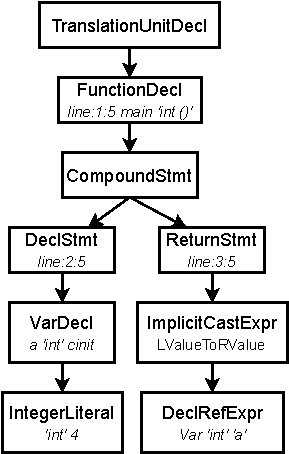
\includegraphics{images/code-to-ast}}
        \caption{Example of converting C++ code to Clang AST. All diagrams show equivalent representation of a small C++ code snippet. The textual representation of the AST shows how information rich each node in the diagrammatic representation is.}
        \label{lst:code-to-ast-example}
    \end{listing}

    \subsection{Pointer Analysis}\label{subsec:pointer-analysis}

    The main capability of the tool is to be able to identify the maximum number of owners a pointer has at all points of the program execution for all pointers in any given program.
    If this number for a given raw pointer is one, then we can go about converting all usages of that raw pointer into a unique pointer.
    If it is more than one then the invariants of a unique pointer cannot be satisfied, and we instead have to use the less performant shared smart pointer.
    A key intuition, mentioned in \autoref{subsec:using-smart-pointers-for-memory-management}, is that a shared pointer can be substituted for most uses of a raw pointer, making it the default fallback.

    A pointer may have more than one owner at a time by copying the pointer to another variable.
    Effectively the address of the underlying region of memory can be accessed through more than one variable, and any accesses of one variable affect the others.
    For example, a pointer may be freed using one variable, and this would invalidate the other variable, causing a memory safety violation if we try to use it.

    We can formalise the notion of copying a pointer by introducing the concept of \emph{escape analysis}.
    Escape analysis is used to determine whether an object \emph{escapes} or is accessible from outside the method or thread that created the object~\cite{Choi1999}.
    It has been used in languages such as Java~\cite{Choi1999} to determine whether an object which is created within a method escapes.
    If it does not, meaning it is only used locally in the method, then it can be allocated on the stack rather than the heap as a performance optimisation.
    Clang also uses escape analysis for a similar kind of optimisation~\footnote{\url{https://github.com/llvm/llvm-project/blob/master/llvm/lib/Analysis/CaptureTracking.cpp}} and also defines the term \emph{pointer capture}.
    A pointer value is captured if the function makes a copy of any part of the pointer that outlives the call.
    We can then see that any pointer that escapes must also be captured since there is no way to refer to an object without being able to determine its address, but not every captured pointer also escapes.
    In \autoref{lst:capture-example} we can see an example where a pointer may be captured but does not escape and in \autoref{lst:escape-example} we see an example of an escaped pointer.

    \begin{listing}
        \inputminted{c++}{code/capture-example.cpp}
        \caption{The pointer is captured in isOdd since the pointer is used for a value that outlives its call, but does not escape since the value of the pointer is not stored anywhere outside the function or thread}
        \label{lst:capture-example}
    \end{listing}

    \begin{listing}
        \inputminted{c++}{code/escape-example.cpp}
        \caption{The pointer is both captured and escapes since the pointer and the value it points to outlive the call of the function and become accessible by any other method or thread as it is copied to a global variable}
        \label{lst:escape-example}
    \end{listing}

    We can now see that invariant of the unique pointer are only violated in two conditions:
    \begin{itemize}
        \item If a pointer escapes, then we do not know where or how the pointer may be used, so we must take a conservative approach and assume the pointer no longer has at most a single unique owner.
        \item If a pointer is does not escape but is captured more than once, then it cannot be a unique pointer.
        The case where a pointer is captured exactly once is a special case that we can model as a move of a unique pointer.
    \end{itemize}

    \subsubsection{Escape Analysis Algorithms}\label{subsubsec:escape-analysis-algorithms}

    Now that we have defined how escape analysis can be used to identify areas of refactoring, we need to identify a suitable algorithm.

    The escape analysis algorithm described by \citet{Choi1999} is used as the default escape analysis algorithm in the Oracle Java Virtual Machine implementation~\footnote{\url{https://docs.oracle.com/en/java/javase/15/vm/java-hotspot-virtual-machine-performance-enhancements.html}} and it is widely cited so it forms the basis of our investigation.
    Due to how similar Java is to C++ and Go in terms of their object-oriented features, it means we can also analyse the escape algorithms used in the Clang and Go compilers.

    \citet{Choi1999} introduce the abstraction of a \emph{connection graph} which we will see is also used in other implementations.
    The connection graph captures relationships between heap-allocated objects and object references.
    The graph is used to perform reachability analysis to determine if an object is local to a thread or method.
    Most importantly, this abstraction allows for a powerful interprocedural analysis to be performed.

    The CG is a directed graph $CG = (N_{o} \cup N_{r}, E_{p} \cup E_{d} \cup E_{f})$ where $N_{o}$ is the set of objects.
    $N_{r}$ is the set of reference nodes which include local variables, parameters, fields and global reference variables.
    $E_{p}$ is the set of points-to edges which exist between a reference node that points to object node.
    $E_{d}$ is the set of deferred edges, where a deferred edge from one node $p$ to node $q$ signifies it points to what $q$ points to.
    $E_{f}$ is the set of of all edges between objects that are a field of another object.
    We can see in \autoref{fig:connection-graph-choi} how a connection graph would be constructed for simple Java statements.

    \begin{figure}
        \centering
        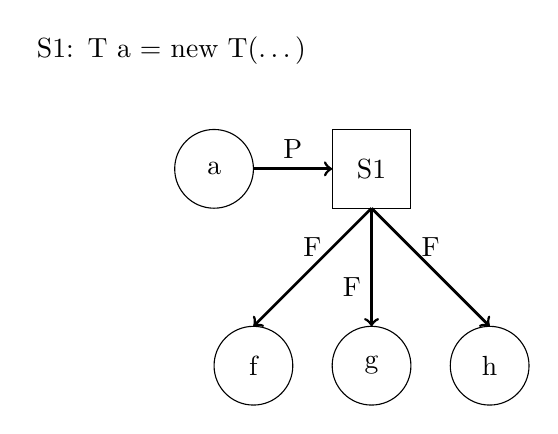
\begin{tikzpicture}[scale=0.5]
            \draw (0, 0) circle (1) node{a};
            \draw[->, line width=1pt] (1, 0) -- node[above] {P} (3, 0);
            \draw (3, -1) rectangle node{S1} (5, 1);

            \draw (1, -5) circle (1) node{f};
            \draw (4, -5) circle (1) node{g};
            \draw (7, -5) circle (1) node{h};
            \draw[->, line width=1pt] (4, -1) -- node[above] {F} (1, -4);
            \draw[->, line width=1pt] (4, -1) -- node[below left] {F} (4, -4);
            \draw[->, line width=1pt] (4, -1) -- node[above] {F} (7, -4);

            \node[text width=4.5cm] at (0, 3) {S1: T a = new T(\ldots)};
        \end{tikzpicture}
        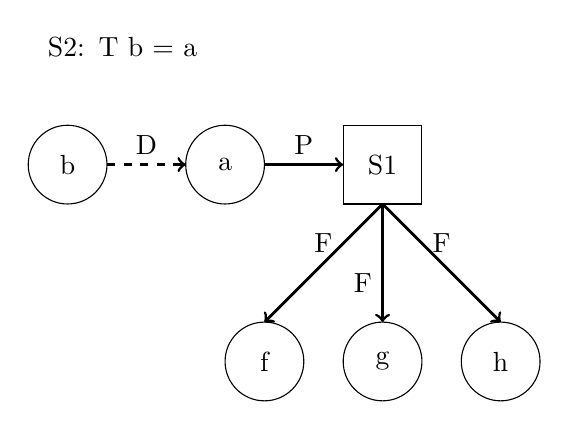
\begin{tikzpicture}[scale=0.5]
            \draw (-4, 0) circle (1) node{b};
            \draw[->, line width=1pt, dashed] (-3, 0) -- node[above] {D} (-1, 0);
            \draw (0, 0) circle (1) node{a};
            \draw[->, line width=1pt] (1, 0) -- node[above] {P} (3, 0);
            \draw (3, -1) rectangle node{S1} (5, 1);

            \draw (1, -5) circle (1) node{f};
            \draw (4, -5) circle (1) node{g};
            \draw (7, -5) circle (1) node{h};
            \draw[->, line width=1pt] (4, -1) -- node[above] {F} (1, -4);
            \draw[->, line width=1pt] (4, -1) -- node[below left] {F} (4, -4);
            \draw[->, line width=1pt] (4, -1) -- node[above] {F} (7, -4);

            \node[text width=4.5cm] at (0, 3) {S2: T b = a};
        \end{tikzpicture}
        \caption{A simple connection graph. Boxes indicate object nodes and circles indicate reference nodes (including field reference nodes). Solid edges indicate points-to edge, dashed edges indicate deferred edges, and edges from boxes to circles indicate field edges~\cite{Choi1999}}
        \label{fig:connection-graph-choi}
    \end{figure}

    For each node, we associate a state of either \emph{NoEscape}, \emph{ArgEscape} or \emph{GlobalEscape}.
    \emph{NoEscape} means that the object does not escape the method in which it was created.
    \emph{ArgEscape}, with respect to a method, means that the object escapes that method via the method arguments or return value,
    but does not escape the thread in which it is created.
    Finally, \emph{GlobalEscape} means that the object is regarded as escaping globally.
    The initial state for each global node is \emph{GlobalEscape} and \emph{NoEscape} for all other nodes, unless otherwise stated.

    The escape analysis is executed through the construction of intraprocedural connection graphs for each method call.
    We then proceed with creating the interprocedural graph by using the connection graph of the callee to update the connection graph of the caller.

    At the completion of the escape analysis, all objects which are marked NoEscape and cannot be reached by any node whose state is not \emph{NoEscape} do not escape and are local to the thread in which they are created.
    We show in \autoref{subsubsec:interprocedural-analysis} how we can adapt this algorithm to check if the invariants defined in \autoref{subsec:pointer-analysis} are met.

    Go is another language that uses a escape analysis to allocate objects on the stack rather than the heap.
    Their escape analysis algorithms is not defined in the specification of the language, however we can look at the source code~\footnote{\url{https://github.com/golang/go/blob/master/src/cmd/compile/internal/gc/escape.go}} to determine what algorithm they use.
    Fortunately the comments give a summary of their algorithm, which involves constructing a weighted graph where vertices represent variables, and edges represent assignments between variables.
    They walk the graph, looking for assignment paths that violate the invariants of a variable being allocated on the stack and mark those as requiring heap allocation
    We can see that this approach is highly similar to the use of connection graphs by \citet{Choi1999}, however there is lacking documentation on how they perform interprocedural analysis so their analysis is perhaps weaker.

    Finally, LLVM also uses escape analysis to remove any unnecessary heap allocations.
    The escape analysis algorithm is also not formally defined, however we can also look at the source code~\footnote{\url{https://github.com/llvm/llvm-project/blob/master/llvm/lib/Analysis/CaptureTracking.cpp}}.
    We see that the \mintinline{c++}{PointerMayBeCaptured} function uses the fact that the single static assignment (SSA) in the LLVM IR allows for efficient creation of definition-usage chains.
    For any defined value, such as a value initialising a variable, we can traverse all its usages, such as copying to another variable.
    To determine if an object escapes, we analyse all its usages, and all their usages and so on.
    For each usage, we then determine if it is an instruction which would cause the object to escape.
    This leads to a roughly similar analysis as the work by \citet{Choi1999} when considering the intraprocedural analysis alone, as we informally explore a graph of the nodes that represent objects and nodes that obtain references to objects by using the original value in a copy instruction.
    However, its assumption about different instructions are conservative, and it also has no interprocedural analysis, making it the weakest analysis so far.

    \subsection{Memory Safe Languages}\label{subsec:rust}

    There have been many proposed systems languages such as Rust~\cite{Balasubramanian2017}, Swift~\footnote{\url{https://developer.apple.com/swift/}}, D~\footnote{\url{https://dlang.org/}}, Nim~\footnote{\url{https://nim-lang.org/}} or Ada (SPARK)~\footnote{\url{https://adacore.com/}}.
    Yet none of these have arguably become mainstream alternatives to C and C++, with Rust and Ada coming closest.

    Swift remains mostly a language for application creation in the the Apple MacOS and iOS environments, however it has seen some usage for system programs by companies such as IBM~\footnote{\url{https://github.com/ibm-swift}}.
    Ada or its subset language SPARK are used extensively in certain industries to create verifiable programs for critical systems such as in avionics.
    It is perhaps most well-know for being used in the F-22 fighter aircraft~\cite{Malas1997}, however the use of Ada for those systems show its other weakness in productivity time as it was the cause for several delays in the project, and so it largely remains unused in areas which do not call for such meticulous safety.

    Rust has been the most popular language in attracting widespread adoption as a systems language.
    Its popularity could be quantified by considering that it is being considered for use in writing Linux kernel modules~\footnote{\url{https://lore.kernel.org/lkml/CAKwvOdmuYc8rW_H4aQG4DsJzho=F+djd68fp7mzmBp3-wY--Uw@mail.gmail.com/T}}, which cannot be said for C++.
    Following the advice given by many that most systems programs should be written in Rust from now on, we see a potential future usage of our work in the creation of a C++ to Rust transpiler.

    Whilst the automatic refactoring of raw pointers into smart pointers solves some memory issues, the language still offers other ways to break memory safety.
    Equivalent idiomatic Rust would be able to find some of these other errors at compile time.
    A C++ to Rust transpiler would be a much larger undertaking, however we can envision how our project could be helpful.
    Rust affine types~\cite{Balasubramanian2017} are semantically equivalent to C++ unique pointers, in that all values have a single unique owner at any point.
    Therefore our work can identify which pointers are unique and which are not, and those that are not cannot be transpiled into idiomatic Rust.

    \subsubsection{Garbage Collected Languages}

    Garbage collected languages encompass some of the most popular programming languages such as Java or Go.
    They are considered to be simpler languages than C++ since they remove the need for manual memory management by the programmer.
    In C++, if memory is improperly freed, it gets leaked and can eventually cause out of memory errors.
    Garbage collectors instead run periodically and scan the memory of the program to find objects in memory which were allocated but are no longer used anymore and then free the leaked objects.
    Languages such as Java~\cite{Tauro2012} use this fully by allocating almost every object on the heap and not freeing any object, instead relying on the garbage collector to clean up.
    They are therefore considered to be easier and more productive to use.

    Garbage collection does also exist for C++ such as the Boehm-Demers-Weiser conservative garbage collector~\cite{Boehm2002}.
    So why is garbage collection not used in every language?
    Garbage collection is not zero-cost as the garbage collection algorithm typically stops the execution of the running program to clean up the memory.
    This means that latency or pauses are introduced to every program, and can occur at any point in the execution of the program, such as during the hot path of the program.

    This has led to garbage collected languages being unsuitable for use in real time systems such as operating systems, as it would be undesirable to have seemingly random latency when interacting with the system.
    There has been research in modern garbage collection algorithms such as ZGC~\cite{Liden2018} and Shenandoah~\cite{Flood2016} for Java which aim to reduce the number and duration of pauses where the garbage collector runs, increasing the responsiveness of the Java virtual machine.
    However, even with much reduced duration of pauses, it may still be unsuitable for some systems with strict latency requirements.

    \subsection{Existing Tools and Research}\label{subsec:existing-tools-and-research}

    As mentioned in \autoref{subsec:do-smart-pointer-solve-memory-management?}, our work closely aligns with the research done around \emph{source code rejuvenation}.
    We believe research in this area is going to increase, as languages move and evolve much quicker than can be supported in enterprise environments, which is supported by the fact that other relevant work has been completed on this subject.

    First and foremost, we have evidence that this is a problem that actually exists in industry through a paper by \citet{Wright2013} which describes a tool used in Google for running such rejuvenations across a large codebase and shows an example of running a simple rejuvenation of upgrading an API call.
    They only use Clang for the parsing of code into an AST and traversing the tree to identify and perform simple refactorings.
    This allows for less complex refactorings, however it also allows for a flexible design to implement different refactorings using the same tool, rather than the focus we have for a single specific refactoring goal.

    Secondly, there has been separate academic research into rejuvenation tools such as the work by \citet{Huck2016} and \citet{Kumar2012}.
    The former also uses the Clang and AST driven approach that we have described in \autoref{subsec:clang-and-llvm} and by \citet{Wright2013}, while the latter uses a representation called IPR~\cite{Dos2011}, which is a general and efficient data structure for representing C++ programs.
    We have not evaluated IPR as a representation to use instead of the Clang AST, but we can however comment that whilst we appreciate the aim of the project to create a efficient and compiler-independent representation, the greater amount of documentation that Clang has, as well as it being the choice of several other successful projects leads us to believe that we will not lose any effectiveness in our use of it.


%%%%%%%%%%%%%%%%%%%%%%%%%%%%%%%%%%%%%%%%%%%%%%%%%%%%%%%%%%%%%%%%%%%%%%%%%%%%%%%%%%%%%%%%%%%%%%%%%%%%%%%%%%%%%%%%%%%%%%%%


    \section{Proposed Approach}\label{sec:proposed-approach}

    \subsection{Current Progress}\label{subsec:current-progress}

    As mentioned in \autoref{subsec:clang-and-llvm}, we plan on using Clang for parsing C++ code into an AST and LLVM IR for the analysis.
    We can traverse the AST and look for nodes of interest, such as variable declaration nodes.
    Given a node in the AST, we can find its equivalent declaration in the IR\@.
    This is mainly possible since we can see in \autoref{lst:code-to-ast-ir} that the variable names can be matched from the code and therefore AST to the IR\@.

    \begin{listing}
        \inputminted{c++}{code/code-to-ast.cpp}
        \inputminted[fontsize=\footnotesize]{llvm}{code/code-to-ast-summary.ll}
        \caption{The LLVM IR representation of a small C++ code snippet. Listing has been summarized for clarity.}
        \label{lst:code-to-ast-ir}
    \end{listing}

    We can then apply escape analysis for this particular value declaration, which will give us a boolean \mintinline{c++}{true} or \mintinline{c++}{false} result.
    Based on the returned value, we know if the value does not escape and if so, we can refactor all the uses of this value.
    This will involve changing the type of the initial declaration, its definition, as well as removing all deletions of the pointer, which can be seen in \autoref{lst:manual-leak} and \autoref{lst:first-example-unique}.
    The diagram in \autoref{fig:design} shows a visual representation of this proposed design.

    \begin{figure}
        \centering
        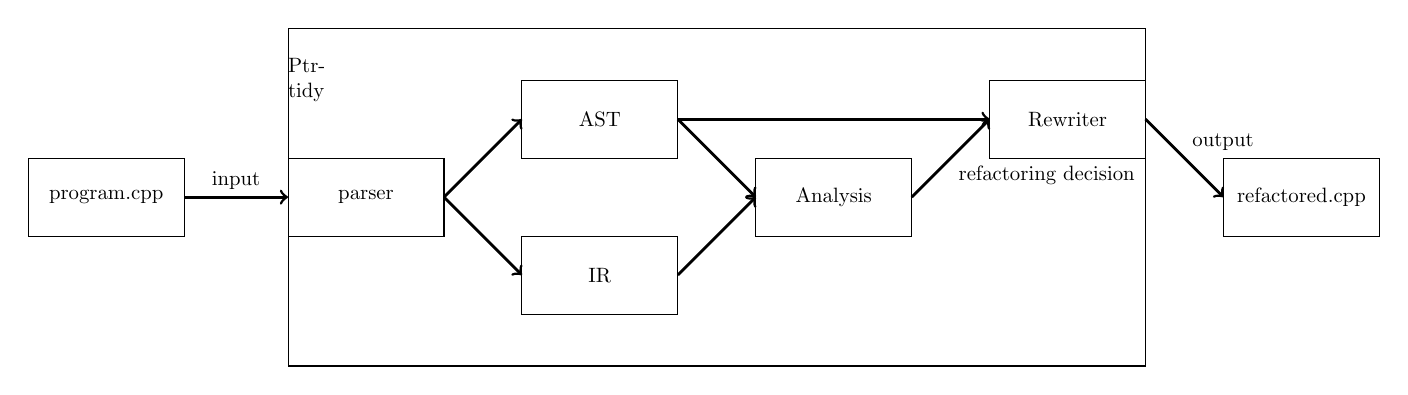
\begin{tikzpicture}[scale=0.33, every node/.style={scale=0.75}]
            \draw (0,0) rectangle node{program.cpp} (6, 3);
            \draw (10, 0) rectangle node{parser} (16, 3);
            \draw[->, line width=1pt] (6, 1.5) -- node[above] {input} (10, 1.5);

            \draw (19, 3) rectangle node{AST} (25, 6);
            \draw (19, 0) rectangle node{IR} (25, -3);
            \draw[->, line width=1pt] (16, 1.5) -- (19, 4.5);
            \draw[->, line width=1pt] (16, 1.5) -- (19, -1.5);

            \draw (28, 0) rectangle node{Analysis} (34, 3);
            \draw[->, line width=1pt] (25, 4.5) -- (28, 1.5);
            \draw[->, line width=1pt] (25, -1.5) -- (28, 1.5);

            \draw (37, 3) rectangle node{Rewriter} (43, 6);
            \draw[->, line width=1pt] (25, 4.5) --  (37, 4.5);
            \draw[->, line width=1pt] (34, 1.5) -- node[below right, text width=3cm] {refactoring decision} (37, 4.5);

            \draw (46, 0) rectangle node{refactored.cpp} (52, 3);
            \draw[->, line width=1pt] (43, 4.5) -- node[above right] {output} (46, 1.5);

            \draw (10, -5) rectangle (43, 8);
            \node[text width=0cm] at (10, 6) {Ptr-tidy};

        \end{tikzpicture}
        \caption{Proposed design of Ptr-tidy tool. Parser is the Clang C++ parser which produces an AST and IR representation of the input code. Analysis is the chosen escape analysis algorithm. It produces a decision of whether the pointer is suitable for refactoring, and passes this to the refactoring component which rewrites the code using smart pointers to produce the safer output program.}
        \label{fig:design}
    \end{figure}

    This design is largely inspired by the componentised design of LLVM~\cite{Lattner2004} and brings several advantages.
    Firstly the analysis is performed on the IR and so it could be reused by the frontend of a different language and not just necessarily Clang.
    Secondly this also enables us to flexibly test different algorithms as the C++ specific parsing and refactoring code is not affected by the choice or power of the analysis.

    This design has been already used to create a prototype of the tool~\footnote{\url{https://github.com/a-usov/ptr-tidy/tree/c44e67022ba5fa2b3a541f4e730230c1e378e46e}}.
    The prototype shows that combining the AST and IR is viable and uses the already implemented LLVM escape analysis on variable declarations.
    It also shows how Clang library allows for easy refactoring since the AST stores all source text and line numbers, making text substitution trivial.
    Substitution of AST nodes rather than source text substitution has not been explored, however this because Clang documentation states that generally the AST should remain immutable.

    The prototype does not currently combine the analysis with the refactoring, which will be the next logical step.
    The source refactoring is also not fully implemented, and is currently only a proof-of-concept.
    However, \autoref{lst:prototype} shows an example output of running the prototype on a small code block, and it shows how the core idea of the project is achievable.

    \begin{listing}
        \inputminted{c++}{code/prototype-input.cpp}
        \inputminted{text}{code/prototype-output.txt}
        \caption{Output from using prototype tool on a small program. We see the analysis of the variables in the code, as well as source code refactoring to use smart pointers. Analysis and refactoring has not yet combined as $b$ should not be refactored since the analysis identifies it as being captured, due to not being able to analyse across function boundaries.}
        \label{lst:prototype}
    \end{listing}

    \subsection{Proposed Further Work}\label{subsec:proposed-further-work}

    As mentioned in \autoref{subsec:current-progress}, further work needs to be completed to create a fully capable first version of the tool.
    This will involve completing the code refactoring component and combining this with the analysis.
    This first version will allow us to use the tool for initial benchmarking, as described in \autoref{subsec:benchmarking}, and this will also likely expose unhandled edge-cases, allowing us to refine the design before moving on to completing more complex analyses.
    This means we can quickly achieve a minimum viable product.

    Afterwards, the focus will be on improving the analysis by implementing an interprocedural analysis, as we envision that the existing LLVM analysis will give us poor results.
    This is because pointers are more often used across function boundaries, as otherwise the programmer could have used a stack variable instead.

    \subsubsection{Interprocedural Analysis}\label{subsubsec:interprocedural-analysis}

    We propose using a modified version of the escape analysis algorithm by \citet{Choi1999} to identify if the proposed invariants in \autoref{subsec:pointer-analysis} are violated.
    The original algorithm already determines whether a pointer escapes or not, however it cannot determine what the maximum number of unique owners a pointer will have throughout the execution of the program.
    We can reuse their idea of the connection graph and add an extra condition.

    In \autoref{fig:connection-graph-choi} we can see that when we copy a pointer, a new reference node with a deferred edge is created, pointing to the original pointer.
    Therefore if each reference node has at most one incoming edge, then we know that each pointer is copied at most once, and therefore only transfers ownership once.
    This therefore means that the value will have at most one unique owner throughout program execution.
    This relies on careful modeling where using pointers as function arguments is modelled as the creation of new reference nodes, which can be correctly modelled in C++ as it has pass-by-value semantics.

    Such an algorithm should give us better results as it will be able to determine whether pointers which are returned from functions escape, as this is a case which the intraprocedural analysis cannot determine and has to take a conservative approach in assuming it escapes.

    \subsection{Shared Pointer Cycle Analysis}\label{subsec:shared-pointer-cycle-analysis}

    There is an emphasis in the project that the refactored program should not differ in runtime behaviour.
    The implementation of shared pointers in the C++ standard library however cause a possible issue to this aim.
    First of all, shared pointers are implemented using reference counting~\cite{Collins1960}, so there is already a performance detriment compared to raw pointers.
    We choose to omit performance detriments, as they are likely to be marginal, however we will benchmark if any exists.

    The issue that we are concerned with are functional requirements of programs, specifically that in some cases, shared pointers will fail to free memory.
    This occurs when shared pointers are used to create reference cycles, such as can be seen in \autoref{lst:reference-cycle}.
    This would go against our aim of improving memory safety.

    We therefore propose to have an analysis stage for checking for reference cycles.
    If we identify a cycle, we do not perform any refactoring and leave the code as it was.
    To identify cycles, we create a type graph of all the user defined types, and we can use depth first traversal to identify a cycle.
    We do this by marking visited nodes in the graph as visited, and if during the traversal an adjacent node to the current node being analysed is already marked as visited, then a cycle exists.

    \begin{listing}
        \inputminted{c++}{code/reference-cycle.cpp}
        \caption{The Person class is used to create a reference cycle. To deallocate the person field in bob, the alice object must be first deallocated. To do so, the bob object in must be deallocated first and so on, meaning the memory will never get deallocated.}
        \label{lst:reference-cycle}
    \end{listing}

    \subsection{Benchmarking}\label{subsec:benchmarking}

    There are several different benchmarks and tests we will perform to analyse the performance and correctness of the tool.
    Firstly, it was mentioned in \autoref{subsec:shared-pointer-cycle-analysis}, we will benchmark our refactored programs against the originals for performance, so see if our refactoring efforts cause a significant detriments.
    Depending on the benchmark program and the effectiveness of the program, the refactoring could only include new unique pointers, which would result in identically performing programs.

    Secondly, where automated test exist for the refactored programs, we will use them to ensure that the logic of the program is unchanged after refactoring.

    Thirdly, we want to analyse how powerful our analysis is in identifying all opportunities in upgrading pointers to unique pointers.
    Our tool has to be conservative in some of its assumptions so might not be able to identify all opportunities.
    We can measure the amount of unique pointers compared to the number of all pointers.
    However, this number will fluctuate massively depending on what program it is run on, such as one handling resources such as files.
    Therefore, the method we propose is to measure the performance of our tool against human refactored test cases, to see how much worse our analysis is compared to human effort.

    % TODO - reference SPEC - find more better benchmarks
    The programs that will be used for the benchmarking will be the subset of C++ programs in the SPEC CPU benchmark suite, as they will usually be pointer heavy, as well as allowing us to measure any possible performance detriments.


%%%%%%%%%%%%%%%%%%%%%%%%%%%%%%%%%%%%%%%%%%%%%%%%%%%%%%%%%%%%%%%%%%%%%%%%%%%%%%%%%%%%%%%%%%%%%%%%%%%%%%%%%%%%%%%%%%%%%%%%


    \section{Work Plan}\label{sec:work-plan}

    We have performed a risk analysis for the project, our design as well as our work plan, seen in \autoref{fig:gantt}, which outlines a schedule for the completion of this project:

    \subsection{Risk Analysis}\label{subsec:risk-analysis}

    \begin{itemize}
        \item Firstly, the frameworks we have chosen to use, namely LLVM and Clang are mature and enterprise-backed open-source frameworks, and therefore we see no risk in using them for current and any future development,
        \item Secondly, the work plan has been structured in such a way that given any unforeseen setbacks in the project, our existing prototype can be finished without the integration of more complex analyses to provide a minimum viable product which can be used in experimentation and evaluation.
        This ensures that we can answer our research questions for this project.
    \end{itemize}

    \newpage

    \subsection{Gantt Chart}\label{subsec:gantt-chart}

    \begin{figure}[!htb]
        \rotatebox{90}{
        \begin{ganttchart}{1}{14}
            \gantttitle{Work Plan}{14} \ganttnewline
            \gantttitlelist{1,...,14}{1} \ganttnewline
            \ganttgroup{Complete Prototype}{1}{3} \ganttnewline
            \ganttbar{Finish Rewriting Component}{1}{1} \ganttnewline
            \ganttbar{Combine all components into final prototype}{2}{2} \ganttnewline
            \ganttbar{Evaluate final prototype and find edge-cases}{3}{3} \ganttnewline
            \ganttgroup{Benchmark and Data Acquisition}{2}{3}  \ganttnewline
            \ganttbar{Find, setup and test benchmark suite}{2}{3} \ganttnewline
            \ganttgroup{Analysis Algorithm Exploration}{4}{7} \ganttnewline
            \ganttbar{Implement proposed interprocedural analysis}{4}{5}\ganttnewline
            \ganttlink{elem3}{elem7}
            \ganttbar{Evaluate tool with interprocedural analysis}{6}{6} \ganttnewline
            \ganttbar{Implement cycle analysis and evaluate}{7}{7} \ganttnewline
            \ganttgroup{Result Consolidation}{8}{14} \ganttnewline
            \ganttbar{Research Paper Writeup}{8}{14} \ganttnewline
        \end{ganttchart}}
        \caption{A Gantt chart demonstrating the project schedule, broken down over the first
        14 weeks of the year from Monday 11th January until Friday 16th April.
        }
        \label{fig:gantt}
    \end{figure}


%%%%%%%%%%%%%%%%%%%%%%%%%%%%%%%%%%%%%%%%%%%%%%%%%%%%%%%%%%%%%%%%%%%%%%%%%%%%%%%%%%%%%%%%%%%%%%%%%%%%%%%%%%%%%%%%%%%%%%%%


    \bibliographystyle{plainnat}
    \bibliography{proposal}
\end{document}
